\chapter{BIOMOLECULAR SIMULATION: SAMPLING AND FREE ENERGY}

All of the simulation models discussed in Chapter \ref{ch1} use an electrostatic
equation dealing with charges interacting in a vacuum. However, biological
chemistry occurs almost exclusively in an aqueous environment, necessitating the
development of models capable of simulating an aqueous environment for these
systems. In this chapter, we will describe the various methods by which solvent
effects are introduced into simulation, followed by the ensemble sampling
techniques that will be used for the principle studies in this dissertation.

\section{Simulations in the Condensed Phase}

The techniques by which solvation effects can be incorporated into various
computational models can be separated into two groups. The most obvious way is
to include the solvent atoms and molecules directly into the simulation
alongside the system of interest---referred to collectively as \emph{explicit
solvent} methods. While explicit solvent models are the most accurate approach
in principle, they drastically increase the size of the
simulation---simultaneously increasing the cost of the simulation and amount of
sampling required to obtain converged results.

An alternative way to include solvent effects is by modifying the electrostatic
interactions in a system to account for the natural screening that a particular
solvent provides. These approaches are called \emph{implicit solvent} methods
because solvent effects are included in an average way without including the
actual solvent atoms or molecules in the simulation. Simulations employing
implicit solvent models result in smaller simulations in which comformational
sampling converges more rapidly because the solvent degrees of freedom are
already included in a mean field way. However, individual solvent molecules
often play a critical role in the structure and function of biological molecules
and behave very differently than bulk solvent molecules---an effect implicit
solvent models are ill-equipped to handle.

The following sections describe the various implicit and explicit solvent models
commonly used in biomolecular simulations.

\subsection{Implicit Solvent}

One of the most important qualities of a solvent---especially an aqueous
solvent---is its ability to polarize in response to an electric field, thereby
reducing the magnitude of electrostatic interactions across a given distance.
While the na\"ive approach of simply applying the solvent dielectric everywhere
is attractive in its simplicity, solvent-excluded regions should obviously not
be subject to the screening effects of the solvent. For large biomolecules, the
solvent-excluded regions can be very large, so it becomes very important to deal
with these regions effectively.

\subsubsection{Distance-dependent Dielectric}

Among the earliest approaches to account for the different dielectric
environments of a bimolecule interior and bulk solvent introduced a dielectric
constant that changed as a function of the distance between two charged
particles. As the separation between two particles increased, so too did the
likelihood that they were separated by solvent, and so were subject to
dielectric screening effects.

This approach is attractive in its simplicity---it adds little to the
computational cost of the model while retaining the simple,
pairwise-decomposable nature of the electrostatic potential term. A common
equation modeling the dielectric constant is given below in Eq.
\ref{eq2:DistanceDielectric}. \cite{Leach_Book_MolModel_2001}

\begin{equation}
   \varepsilon _ {eff} (r) = \frac {\varepsilon_{bulk} - 1} 2 \left [ (rS) ^2 +
   2rS + 2 \right ] \exp(-rS)
   \label{eq2:DistanceDielectric}
\end{equation}
where $r$ is the distance between the two particles, $\varepsilon_{bulk}$ is the
dielectric constant of the bulk, $\varepsilon_{eff}$ is the effective
dielectric constant at a given particle separation, and $S$ is a free parameter.
Fig. \ref{fig2:DistanceDielectric} plots the resulting curve for
$\varepsilon_{eff}$ from Eq. \ref{eq2:DistanceDielectric} for different values
of the free parameter.

\begin{figure}
   \includegraphics[width=6.5in]{DistanceDielectric.ps}
   \caption{Distance-dependent dielectric for different values of the free
            parameter $S$ in Eq. \ref{eq2:DistanceDielectric}.}
   \label{fig2:DistanceDielectric}
\end{figure}

This effective dielectric constant is then incorporated as $\epsilon$ in Eq.
\ref{eq1:AmberFF2}, and influences the calculated forces due to its dependence
on $r_{i,j}$. One of the biggest weaknesses of distance-dependent
dielectrics is that it treats every atom in the biomolecule as though they are
in the same environment, and the shapes of biomolecules---and their
solvent-excluded volumes---are often highly irregular. That is, two atoms buried
inside the solvent-excluded volume separated by $d$ {\AA} are treated exactly
the same way as two different atoms $d$ {\AA} apart whose interstitial region is
solvent-accessible. Furthermore, because the shapes of biomolecules can vary
greatly from system to system, the `optimal' value for $S$ in Eq.
\ref{eq2:DistanceDielectric} is highly system-dependent. Finally, while the true
dielectric regions are either the value of the bulk solvent or the molecule
interior, a distance-dependent dielectric has a large region corresponding to
unphysical, intermediate values of the dielectric.

For these reasons, the distance-dependent dielectric model is rarely used in
modern simulations, having given way to the more accurate methods like the
Poisson-Boltzmann equation and Generalized Born equation.

\subsubsection{Poisson-Boltzmann}

At the heart of all modern implicit solvent models lies the Poisson equation
\begin{equation*}
   \bigtriangledown \epsilon(\vec{r}) \cdot \bigtriangledown \phi ( \vec{r} ) =
            -4 \pi \rho(\vec{r})
\end{equation*}
where $\phi$ is the electrostatic potential at a given point in space, $\rho$ is
the charge distribution at a given point in space, and $\epsilon$ is the
dielectric constant at a given point in space. The dielectric constant is often
divided into two regions---a region of low dielectric in the solvent-excluded
volume and that of the bulk solvent `outside' the system of interest.
\cite{Cramer_Book_EssentialsCompChem_2004}

The Poisson equation is only valid, however, at zero ionic strength. When mobile
ions are present---as is the case \emph{in vivo} with all biomolecules---the
Poisson equation must be augmented with an appropriate distribution of
counterions. The probability of finding an ion in a particular region of space
is related to its Boltzmann factor $\exp (-\beta q \phi(\vec{r}))$, where $q
\phi(\vec{r})$ is the energy of a point charge in a given electrostatic
potential. Because ions come in pairs with both positive and negative charges,
the Boltzmann probability of finding both types of ions must be included. The
equation for calculating the electrostatic potential in a biomolecular system
with a given solution ionic strength, termed the \emph{Poisson-Boltzmann} (PB)
equation, is shown in Eq. \ref{eq2:PoissonBoltzmann}.
\cite{Cramer_Book_EssentialsCompChem_2004}

\begin{align}
   \bigtriangledown \epsilon(\vec{r}) \cdot \bigtriangledown \phi(\vec{r}) -
      \epsilon(\vec{r}) \lambda(\vec{r}) \kappa^2 \frac{k_B T} {2 q} \exp \left
      ( -\beta q \phi(\vec{r}) \right ) + \epsilon(\vec{r}) \lambda(\vec{r})
      \kappa^2 \frac{k_B T} {2 q}  \exp \left ( \beta q \phi(\vec{r}) \right )
      \right ] & = -4 \pi \rho (\vec{r}) \nonumber \\
   \bigtriangledown \epsilon(\vec{r}) \cdot \bigtriangledown \phi(\vec{r}) -
      \epsilon(\vec{r}) \lambda(\vec{r}) \kappa^2 \frac{k_B T} q \sinh \left (
      \frac {q \phi(\vec{r})} {k_B T} \right ) & = -4 \pi \rho (\vec{r})
   \label{eq2:PoissonBoltzmann}
\end{align}
where $q$ is the charge of the ions (both positive and negative ions are
present), $\lambda(r)$ is a simple switching function that is 0 in
solvent-excluded regions and 1 in solvent-accessible regions, and $\kappa^2$ is
related to the ionic strength as
\begin{equation*}
   \kappa ^ 2 = \frac {8 \pi q ^ 2 I} {\epsilon k_B T}
\end{equation*}

Eq. \ref{eq2:PoissonBoltzmann} is a non-linear, second-order differential
equation in the electrostatic potential that must be solved iteratively until
the desired level of self-consistency in the electrostatic potential is
achieved. The $\sinh$ term in Eq. \ref{eq2:PoissonBoltzmann} may be expanded
using its Taylor series expansion. If the ionic strength is low and the solute
is not highly charged (so $\phi(\vec{r})$ is relatively small), the Taylor
series expansion for $\sinh$ can be truncated after the first term to yield the
much simpler Eq. \ref{eq2:LinearPB} with little loss of accuracy. Eq.
\ref{eq2:LinearPB} is called the \emph{linearized} Poisson-Boltzmann equation
because the Taylor series expansion for $\sinh$ is truncated after its linear
term.

\begin{equation}
   \bigtriangledown \epsilon (\vec{r}) \bigtriangledown \phi(\vec{r}) -
         \epsilon(\vec{r}) \lambda(\vec{r}) \kappa ^ 2 \phi(\vec{r}) = -4 \pi
         \rho(\vec{r})
   \label{eq2:LinearPB}
\end{equation}

The Poisson Equation can be solved for only the simplest systems, like solvating
a point-charge or a conducting sphere with a uniform charge distribution on its
surface. Eq. \ref{eq2:PoissonBoltzmann} or \ref{eq2:LinearPB} must be solved
numerically for complex biomolecules with irregular shapes. A common approach is
to set up a three-dimensional grid surrounding the solute and calculate the
charge distribution on the grid from the partial charges of each solute atom.
The dielectric boundary can be calculated from the solvent accessible surface
\cite{Sitkoff_JPhysChem_1994_v98_p1978}, so each grid point has an associated
charge and dielectric value. The differential equations can then be solved via
finite differences within the defined grid. \cite{Klapper_Proteins_1986_v1_p47}

After the electrostatic potential is calculated via Eq.
\ref{eq2:PoissonBoltzmann}, the free energy is calculated by integrating the
product of the charge distribution and the calculated electrostatic potential
according to
\begin{equation*}
   G = \frac 1 2 \int \rho(\vec{r}) \phi(\vec{r}) d\vec{r}
\end{equation*}
where the $1/2$ factor corrects for double-counting the interactions.  The free
energy of solvation due to solvent polarization is calculated from the
difference in the electrostatic potentials in vacuum and solvent ($\phi_{solv} -
\phi_{vac}$)---a quantity referred to as the \emph{reaction field}.
\cite{Leach_Book_MolModel_2001} The charge-dependent portion of the solvation
free energy then becomes
\begin{equation}
   \Delta G _ {pol} = \frac 1 2 \int \rho(\vec{r}) \left ( \phi_{solv}(\vec{r})
      - \phi_{vac}(\vec{r}) \right ) d\vec{r}
   \label{eq2:ReactionField}
\end{equation}

Models employing implicit solvent via the PB equation have proven
effective in many cases. \cite{Klapper_Proteins_1986_v1_p47,
Gilson_JComputChem_1988_v9_p327, Baker_ProcNatlAcadSci_2001_v98_p10037,
Nielsen_Proteins_2001_v43_p403} However, due to requirements of a fairly dense
grid and the iterative, self-consistent solution of the PB equation, the
computational cost of this model is too high for many applications. Furthermore,
the dielectric function is discontinuous at the boundaries of the
solvent-excluded and solvent-accessible regions, making stable gradients (and
therefore forces) difficult to calculate.
\cite{Wang_ChemPhysLett_2009_v468_p112} Therefore, we now consider a common
approximation to the PB equation called the \emph{Generalized Born} model that
seeks to provide an efficient, analytical alternative than solving the PB
equation.

\subsubsection{Generalized Born}

While the electrostatic potential generated by most charged species cannot be
solved analytically using the Poisson equation, we will consider two simple,
ideal systems that can. The first is a perfect conducting sphere of radius $r$
with a uniform charge distribution. Given a total charge $q$ and using the
Poisson equation to calculate the electrostatic potential induced by the charged
sphere, the polar contribution to the free energy of solvation can be calculated
from Eq. \ref{eq2:ReactionField}, giving the familiar \emph{Born} equation,
shown below. \cite{Cramer_Book_EssentialsCompChem_2004}
\begin{equation}
   \Delta G _ {pol} = - \frac 1 2 \left( \frac 1 {\epsilon_{vac}} - \frac 1
         {\epsilon_{bulk}} \right) \frac {q ^ 2} r
   \label{eq2:Born}
\end{equation}
where $\epsilon_{vac}$ is the dielectric constant of a vacuum, which is unity.
It is shown explicitly here to demonstrate that the dielectric constant of the
solvent-excluded volume in the Poisson equation does not appear in the Born
equation.

If instead of being a perfect conducting sphere with a uniform charge
distribution, the sphere had a perfect dipolar charge distribution, the free
energy of solvation using the Poisson equation would result in the
\emph{Kirkwood-Onsager} equation, shown below.
\cite{Cramer_Book_EssentialsCompChem_2004}
\begin{equation}
   \Delta G _ {pol} = - \frac 1 2 \left ( \frac {2 ( \epsilon - 1 )} {2 \epsilon
         + 1} \right ) \frac {\mu ^ 2} {r ^ 3}
   \label{eq2:KirkwoodOnsager}
\end{equation}
where the $\epsilon$ is the dielectric constant of the bulk solvent and the
dielectric constant of vacuum has simply been replaced by 1.

The \emph{Generalized Born} (GB) formalism for calculating the polar
contribution to the solvation free energy is, as its name would suggest, an
extension of the \emph{Born} solution shown in Eq. \ref{eq2:Born} to complex
molecules with an arbitrary size and shape.
\cite{Still_JAmChemSoc_1990_v112_p6127, Qiu_JPhysChemA_1997_v101_p3005,
Onufriev_JPhysChemB_2000_v104_p3712, Bashford_AnnuRevPhysChem_2000_v51_p129,
Onufriev_JComputChem_2002_v23_p1297}
\citeauthor{Still_JAmChemSoc_1990_v112_p6127} was the first to propose the
method, adjusting the Born equation (Eq. \ref{eq2:Born}) as shown below.
\cite{Still_JAmChemSoc_1990_v112_p6127}
\begin{equation}
   \Delta G _ {pol} = -\frac 1 2 \left( 1 - \frac 1 {\epsilon} \right)
      \sum_{i=1}^N \sum_{j=1}^N \frac {q_i q_j} {f_{GB}}
   \label{eq2:GB}
\end{equation}
where $q_i$ is the charge of atom $i$, $\epsilon$ is the dielectric constant of
the solvent, and $f_{GB}$ is an arbitrary, analytic function of atom positions
designed to calibrate Eq. \ref{eq2:GB} to experiment. The most common form of
$f_{GB}$ devised by \citeauthor{Still_JAmChemSoc_1990_v112_p6127}, and still
used predominantly today, is shown in Eq. \ref{eq2:fGB}.

\begin{equation}
   f_{GB} = \sqrt{r_{i,j}^2 + \alpha_i \alpha_j \exp \left( - \frac {r_{i,j}^2}
            {4 \alpha_i \alpha_j} \right)}
   \label{eq2:fGB}
\end{equation}
where $r_{i,j}$ is the distance between atoms $i$ and $j$ and $\alpha_i$ is
called the effective Born radius of atom $i$ for reasons that will soon be
apparent.

Eq. \ref{eq2:fGB} does not represent a theoretically `correct' choice for
$f_{GB}$, nor has it been shown to be the best choice---in fact it probably is
not. \cite{Onufriev_JChemPhys_2011_v134_p164104} However, it is a good choice
for several reasons. First, Eq. \ref{eq2:fGB} is a simple formula with
analytical gradients---assuming $\alpha_i$ is an analytic function of the
nuclear positions---and can be computed rapidly. More importantly, however, Eq.
\ref{eq2:fGB} has the appropriate limiting behavior.
\cite{Still_JAmChemSoc_1990_v112_p6127} For a single particle---or two identical
point charges separated by a distance of 0---$f_{GB}$ reduces to $\alpha$ and
Eq. \ref{eq2:GB} reduces to the Born equation (Eq. \ref{eq2:Born}) in which the
radius of the `sphere' is the $\alpha_i$. It is for this reason that the
$\alpha_i$ values can be thought of as an `effective' radius. Furthermore, for
two point charges separated by a small distance (\ie smaller than the effective
radii of the two particles) the result agrees with the Kirkwood-Onsager solution
(Eq. \ref{eq2:KirkwoodOnsager}) to within 10\% of the true value.
\cite{Still_JAmChemSoc_1990_v112_p6127}

The next major challenge in solving Eq. \ref{eq2:GB} is calculating the
effective Born radii, $\alpha_i$, for each atom. The effective radius of an atom
reflects the spherically average distance of that atom from the solvent excluded
surface. Calculating the effective radii is particularly challenging because it
must be done rapidly, accurately, and so gradients may be easily computed.
Because GB was developed as an efficient alternative to solving the PB equation,
computationally intensive approaches to calculating the effective radii offer
little advantage over using the more precise PB equation. Furthermore,
\citeauthor{Onufriev_JComputChem_2002_v23_p1297} has demonstrated the importance
of computing effective Born radii accurately,
\cite{Onufriev_JComputChem_2002_v23_p1297} showing that so-called `perfect
radii' reproduce PB results very closely. Finally, gradients are necessary to
perform either geometry optimization or molecular dynamics, and an expression
that lends itself to rapid computation of an accurate gradient is an attractive
feature.

The most common approach to computing the effective radius is called the
\emph{coulomb field approximation}, shown below in Eq. \ref{eq2:CFA}.
\cite{Cramer_Book_EssentialsCompChem_2004}

\begin{equation}
   I _ i = \int _ {\Omega_i} \frac {d^3r} {4 \pi r ^ 4}
   \label{eq2:CFA}
\end{equation}
where $I_i$ is the coulomb field integral for atom $i$ and $\Omega_i$ signifies
the integral is over all space centered on atom $i$. The effective radius is
then computed from this integral using Eq. \ref{eq2:reff}

\begin{equation}
   \alpha _ {i} = \left( \rho _ i ^ {-1} - I _ i \right) ^ {-1}
   \label{eq2:reff}
\end{equation}
where $\rho_i$ is the intrinsic van der Waals radius of atom $i$ and $I_i$ is
the integral from Eq. \ref{eq2:reff}.

As computational power increased and simulations reached longer time scales and
larger systems, however, deficiencies in these equations began to surface,
leading to efforts to improve the calculation of the effective Born radii.
\cite{Onufriev_JComputChem_2002_v23_p1297, Onufriev_Proteins_2004_v55_p383,
Mongan_JChemTheoryComput_2007_v3_p156, Nguyen_JChemTheoryComput_2013_ASAP} The
two approaches that have been implemented in the Amber suite of programs are
briefly described below.

\citeauthor{Onufriev_Proteins_2004_v55_p383} noticed that Eqs. \ref{eq2:CFA} and
\ref{eq2:reff} tended to underestimate the effective radii of buried atoms
because it assumed that interstitial regions of space between atoms were
solvent-filled, despite the fact that they were too small to contain a full
water molecule. \cite{Onufriev_Proteins_2004_v55_p383} As a result, they
modified Eq. \ref{eq2:reff} into the following form:
\begin{equation}
   \alpha _ i = \left[ \rho _ i ^ {-1} - \rho _ i ^ {-1} \tanh \left( a
   \Psi - \beta \Psi^2 + \gamma \Psi^3 \right) \right] ^ {-1}
   \label{eq2:reffOBC}
\end{equation}
where $I_i$ is taken from Eq. \ref{eq2:CFA}, $\Psi = I \rho_i$, and $a$,
$\beta$, and $\gamma$ are fitting parameters. The $\tanh$ function was chosen
because it is infinitely differentiable (analytically) and increases the
effective radii of more deeply-buried atoms while leaving the effective radii of
atoms closer to the surface unchanged. In this way, Eq. \ref{eq2:reffOBC}
maintains the success Eq. \ref{eq2:reff} displayed for small compounds while
improving the behavior of deeply-buried residues.
\cite{Onufriev_Proteins_2004_v55_p383} This GB variant is referred to as
GB\super{OBC} (where OBC comes from the authors Onufriev, Bashford, and Case).

\citeauthor{Mongan_JChemTheoryComput_2007_v3_p156} took a different approach.
While Eq. \ref{eq2:reffOBC} provided uniform scaling for all atoms with a given
degree of burial (as measured by the value of $I_i$ in Eq. \ref{eq2:CFA}),
\citeauthor{Mongan_JChemTheoryComput_2007_v3_p156} adopted an approach based on
geometry. By treating each atom and each solvent molecule as a sphere---a good
approximation for a water molecule---the interstitial space between two solute
atoms that is inaccessible to solvent (Fig. \ref{fig2:Interstitial}) can be
quantified. Because this interstitial region resembles a neck, this model is
referred to as GB\super{neck}. \cite{Mongan_JChemTheoryComput_2007_v3_p156}

\begin{figure}
   \includegraphics[height=6.5in, angle=90, trim=1cm 0.5cm 1cm 0.5cm, clip=true]
                   {Interstitial.ps}
   \caption{Region of space between two atoms $i$ and $j$ of radius $R_i$ and
            $R_j$ that is inaccessible to a spherical solvent molecule of radius
            $R_solv$. This inaccessible region is called the \emph{neck} and is
            shaded gray.}
   \label{fig2:Interstitial}
\end{figure}

The most recent approach by \citeauthor{Nguyen_JChemTheoryComput_2013_ASAP}
involves a re-parametrization of the intrinsic atomic radii ($\rho_i$ in Eq.
\ref{eq2:reff}) for atoms commonly involved in salt bridges and a combination of
the ideas presented in the GB\super{OBC} and GB\super{neck} models described
above. \cite{Nguyen_JChemTheoryComput_2013_ASAP}

\subsubsection{Non-polar Solvation}

The process of solvation can be broken down into two fictitious steps---a
cavitation step in which the solvent is excluded from a region of space equal to
the solute's solvent excluded volume, and a charging step where the
solvent-polarized charge distribution of the solute is inserted into that
cavity. Because the free energy is a state function, this gedanken decomposition
will yield an identical free energy to the true process that occurs in
experiment---assuming of course that each process can be calculated exactly.
The free energies of these two steps are referred to as the non-polar and polar
solvation free energy, respectively.

The Poisson-Boltzmann and Generalized Born equations shown in Eqs.
\ref{eq2:PoissonBoltzmann} and \ref{eq2:GB} are used to compute the polar
solvation free energy (\ie the portion of the free energy derived from the
reaction field). There are several methods for calculating the non-polar
solvation free energy.

Methods for calculating the non-polar contribution to solvation are often
parametrized by assuming that the solvation free energy for extended and
branched alkanes is non-polar in nature. The most common way to calculate
non-polar solvation is to fit a surface tension value to the experimental
solvation free energies of the alkanes.
\cite{Cramer_Book_EssentialsCompChem_2004} This approach can be rationalized
using the idea that the presence of a non-polar solute immersed in solvent
disrupts the solvent-solvent interactions, thereby restricting solvent structure
in the solvation shell surrounding the solute. This effect imposes an entropic
penalty to solvation (that is offset by the polar solvation term for soluble
compounds).  If this was the only source of the `non-polar' solvation free
energy, then its magnitude would vary with the size of the molecule, which is
directly related to its surface area.

Combining this surface-area non-polar solvation term with either the Generalized
Born or Poisson-Boltzmann equations for the polar solvation term results in the
so-called \emph{GBSA} and \emph{PBSA} methods, respectively. One of the most
common methods for calculating the surface area in GBSA molecular dynamics
simulations is called the \emph{linear combination of pairwise overlaps} (LCPO)
method---so-called because it is parametrized by fitting five parameters to the
spherical overlaps of individual atoms. \cite{Weiser_JComputChem_1999_v20_p217}
The chief advantage of LCPO is that it provides an efficient way to calculate
surface areas using an analytical formula whose derivatives can be easily
calculated for use in molecular dynamics.

\subsection{Explicit Solvent}

While the implicit solvent methods described above are useful ways of
incorporating solvation effects in molecular simulations, all solvent effects
are accounted for in an average way. Therefore, individual water molecules that
play structurally important roles in biomolecules are not treated well by either
PB or GB methodologies. In such cases, it is advantageous to include the solvent
molecules explicitly in the simulation. Explicit solvent significantly increases
the cost of the simulation by adding a large number of atoms to the system, but
should improve the accuracy by creating a model closer to reality.

A large drawback when adding explicit solvent, however, is the fact that modern
simulations at an atomic resolution (\ie where all atoms are treated explicitly)
are limited to, at most, $10^8$ atoms, \cite{100M_Stupid} although simulations
between $10^5$ to $10^6$ atoms are more reasonable. Macroscopic systems, on the
other hand, contain on the order of $10^{23}$ atoms---a number far outside the
range of possibility for modern hardware, so our simulations must be scaled down
to a microscopic size.

As a demonstration, the hairpin ribozyme is a biomolecule that contains roughly
\mbox{2 100} atoms. Adding only \mbox{22 000} water molecules---enough to create
a 20 {\AA} spherical solvent buffer around the ribozyme---increases the
simulation size to roughly \mbox{90 000} atoms. It is quite clear, therefore,
that even on the largest supercomputers, we can only model a microscopic droplet
in explicit solvent. At such small sizes, the ratio of surface area to volume
for these minuscule droplets is astronomically large, and water molecules at the
solvent-air interface behave quite differently from those molecules in bulk
solvent that is typically encountered experimentally.

While early approaches of applying a `cap' potential---an artificial biasing
potential penalizing solvent that diffuses too far away from the solute---helped
overcome some surface effects like evaporation, it made direct comparison to
experiment dubious. A major breakthrough in explicit solvent calculations came
with the introduction of periodic boundary conditions. \cite{Allen_Tildesley}

\subsubsection{Periodic Boundary Conditions}

To emulate bulk solution behavior using a system composed of a tractable number
of atoms, we impose periodic boundary conditions (PBC) on the system,
replicating it infinitely in every dimension. In such a system, each atom
interacts with all other atoms in all other simulation cells---including its own
periodic images. \cite{Allen_Tildesley} A two-dimensional illustration of PBC is
shown in Fig. \ref{fig2:PBC} for a rectangular unit cell illustrating these
ideas.

A practice commonly adopted in PBC simulations in which each atom interacts
directly with only a single image of every other atom---specifically the nearest
image---is called the \emph{minimum image convention}. The minimum image
convention is employed to simplify the problem, but also imposes a limit to the
range of calculated interactions. Specifically, the non-bonded interactions do
not extend beyond half the length of the shortest side of the unit cell.
Employing the minimum image convention, the energy calculated for a system with
PBC is the energy of a single unit cell in the field generated by all other
periodic cells. The challenge is how to calculate the non-bonded interactions
for every atom in the system. The common approaches employed in biomolecular
simulation is explored in the next three sections.

\begin{figure}
   \includegraphics[height=6.5in, angle=90, trim=0.7cm 3cm 0.7cm 3cm, clip=true]
                   {PBC.ps}
   \caption{Periodic simulation in two dimensions with a rectangular unit cell.
            The maximum permissible cutoff (r\sub{cut}) for the minimum image
            convention is shown with a blue dotted circle centered on particle 1
            in the first box.}
   \label{fig2:PBC}
\end{figure}

\subsubsection{Cutoff Methods}

The simplest approach to calculating non-bonded interactions is to employ a
simple cutoff that is smaller than half the length of the shortest side of the
unit cell---\ie all non-bonded interactions between atoms closer than the cutoff
are included and all those between atoms greater than the cutoff are neglected.
Because the common forms of the non-bonded potential decay as the distance
between atoms increases (see Eqs. \ref{eq1:ElectrostaticInteractions} and
\ref{eq1:LennardJones}), interactions between distant atoms are significantly
smaller than interactions between nearby atoms. The non-bonded interactions are
modeled as the simple piecewise function shown in Eq. \ref{eq2:cutoff}.

\begin{equation}
   U^{\prime}(\vec{x}_{i,j}) = \left \{
   \begin{array}{lr}
      U(\vec{x}_{i,j}) & : \left | \vec{x}_{i,j} \right | < x_{cut} \\
      0 & : \left | \vec{x}_{i,j} \right | > x_{cut}
   \end{array}
   \right.
   \label{eq2:cutoff}
\end{equation}

While conceptually simple and computationally efficient, simple cutoffs suffer
from a severe limitation. The potential, and therefore the force, encounters a
discontinuity at the cutoff distance, shown in Fig.
\ref{fig2:Cutoff}A. This discontinuity results in simulations that do not
conserve energy and leads to numerous, non-physical artifacts.
\cite{Schreiber_JMolBiol_1992_v228_p909, Schreiber_Biochemistry_1992_v31_p5856,
Saito_JChemPhys_1994_v101_p4055, Auffinger_ChemPhysLett_1995_v234_p413,
Cheatham_JAmChemSoc_1995_v117_p4193, Feller_JPhysChem_1996_v100_p17011,
Patra_BiophysJ_2003_v84_p3636} This effect is particularly pronounced for
electrostatic interactions---a very long-range potential of the form $1/r$. This
function decays so slowly, in fact, that $\sum_{i=1}^{\infty} 1/r = \infty$.
Two monovalent ions must be separated by ~332 {\AA} before their interaction
energy drops to 1 kcal/mol. Such a cutoff would require a unit cell size at
least 664 {\AA} on each edge containing $\sim 10^7$ water molecules.

Given the need to improve the behavior of the non-bonded potentials near the
cutoff distance, two popular modifications to the simple cutoff approach were
introduced---a smooth switching function and a shifting function. The switching
function approach applies a smooth function at a given distance that satisfies
the following criteria: a) the potential and its gradient is continuous
everywhere, b) the short-ranged form of the potential is unchanged, and c) the
potential approaches 0 at the cutoff. Eq. \ref{eq2:cutoff} is an example of a
very simple switching function in which the original potential is multiplied by
1 when the interparticle distance is less than the cutoff and 0 otherwise. Of
course, this switching function does not obey either the a) or c) conditions
listed above. An example of a smooth switching function is shown in Fig.
\ref{fig2:Cutoff}B. \cite{Steinbach_JComputChem_1994_v15_p667}

The second family of methods commonly employed are so-called shifting functions
since the potential is modified by `shifting' the potential up such that the
value of the potential becomes zero at the cutoff distance.
\cite{Steinbach_JComputChem_1994_v15_p667, Allen_Tildesley} Simply shifting the
potential, though, is not enough for MD simulations, since the force will remain
unchanged and still faces a discontinuity at the cutoff. Therefore, the shifting
function often contains a force-shifting component, as shown in Eq.
\ref{eq2:ShiftingFunction}. \cite{Allen_Tildesley} The effect of the shifting
function is shown in Fig. \ref{fig2:Cutoff}C.

\begin{equation}
   U_s(\vec{r}_{i,j}) = \left\{
   \begin{array}{lr}
      U(\vec{r}_{i,j} - U(\vec{r}_{cut}) - \left( \frac {dU(\vec{r}_{i,j})}
        {d\vec{r}_{i,j}} \right) _ {\vec{r}_{i,j} = \vec{r}_{cut}}
        (\vec{r}_{i,j} - \vec{r}_{cut}) & \vec{r}_{i,j} \lt \vec{r}_{cut} \\
      0 & \vec{r}_{i,j} \geq \vec{r}_{cut}
   \end{array}
   \right.
   \label{eq2:ShiftingFunction}
\end{equation}

\begin{figure}
   \includegraphics[height=6.5in, angle=90]{Cutoff.ps}
   \caption{Effects of various 16 {\AA} cutoff schemes on the electrostatic
   interaction of two monovalent ions with opposite charges. A) shows the
   effect of imposing a hard cutoff. B) shows a typical switching function
   starting at 8 {\AA}. C) shows a typical shifting function for the
   electrostatic potential. The energies as a function of distance are shown in
   the top 3 plots and the forces as a function of distance are the bottom 3
   plots.}
   \label{fig2:Cutoff}
\end{figure}

\subsubsection{Ewald Summation}

Ideally, simulations in the condensed phases would be performed \emph{without}
truncating electrostatic interactions at all. The full electrostatic interaction
for a net neutral unit cell takes the functional form $\sum_{i=1}^N (-1)^i / i$,
since there are an equal number of charges of both signs. This sum is
\emph{conditionally convergent}, meaning that, while its value converges to a
finite value, the value that it converges to depends on the order in which the
terms are summed. \cite{Allen_Tildesley} A natural choice for ordering the
summation of the infinite number of electrostatic interactions with particle $i$
is by summing all of the electrostatic interactions with each particle $j$ in
every unit cell extending radially from the unit cell containing $i$. This
approach is shown diagrammatically in Fig. \ref{fig2:PeriodicCells}.
\cite{Allen_Tildesley}

\begin{figure}
   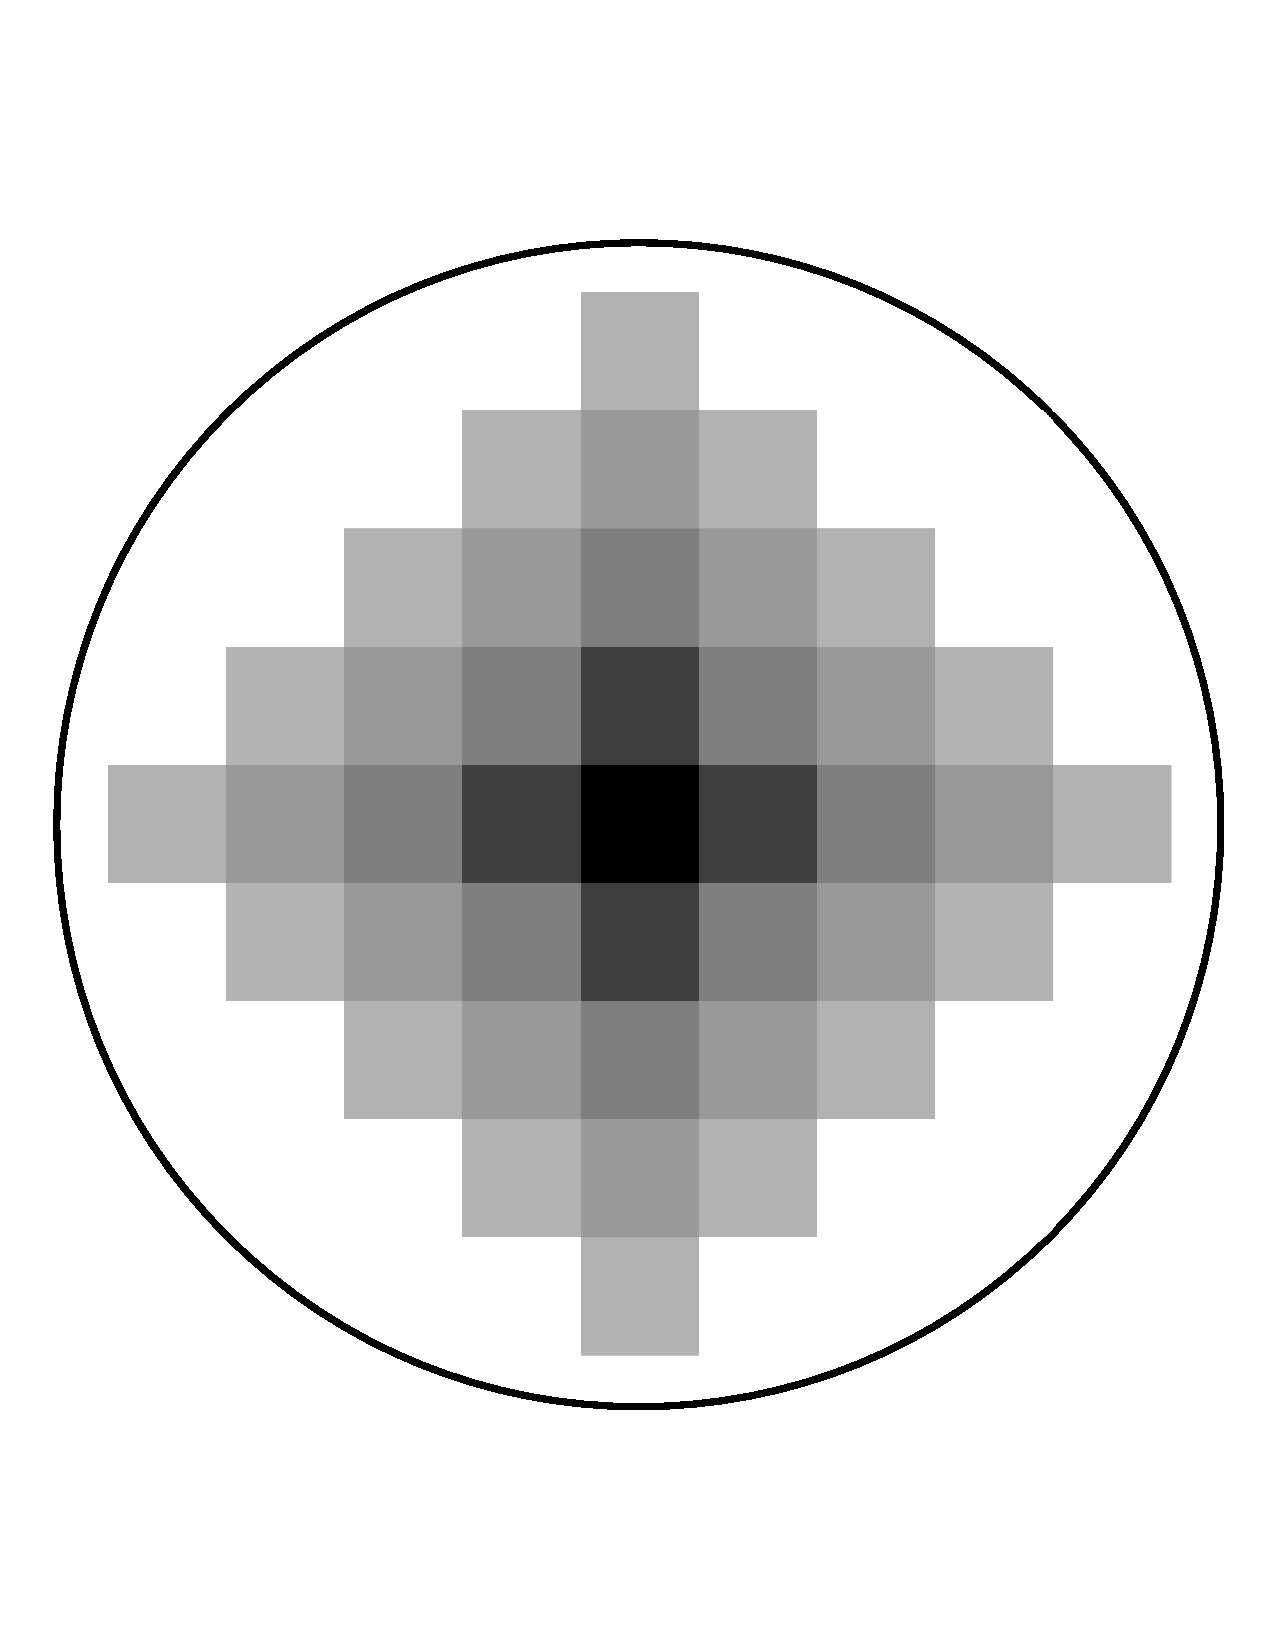
\includegraphics[height=4in, angle=90, trim=0.1cm 2cm 0.1cm 2cm, clip=true]
                    {PeriodicCells.ps}
   \caption{Periodic cells added in a spherical shape radially from the central
            unit cell. The progression from darker to lighter cells shows the
            order in which interactions are accumulated in the sum of the
            electrostatic interactions (with the darker cells being added before
            the lighter ones). The example, adapted from
            \citeauthor{Allen_Tildesley}, is shown in two dimensions, but can
            be trivially extended to three dimensions. \cite{Allen_Tildesley}}
   \label{fig2:PeriodicCells}
\end{figure}

In 1921, \citeauthor{Ewald_AnnPhys_1921_v64_p253} devised a method whereby the
electrostatic interactions between an ion and all of its periodic images in a
crystal lattice could be computed according to the technique presented in Fig.
\ref{fig2:PeriodicCells}. \cite{Ewald_AnnPhys_1921_v64_p253} The same approach
can be used for simulations in the condensed phase when PBC are used.  The
technique, called the Ewald sum, utilizes a trick to cause the electrostatic
interactions between particles to decay arbitrarily rapidly, allowing the
interactions to be truncated at a distance where the interactions themselves are
negligible. To do this, a Gaussian charge distribution is centered at each point
charge whose integral is the same magnitude as the point charge around which it
is centered, but with opposite sign (Fig. \ref{fig2:Ewald}). Given a width of
the Gaussian distribution $\alpha$, the functional form of the neutralizing
charge distribution is shown in Eq. \ref{eq2:NeutralizingDistribution}.

\begin{equation}
   \rho_i(r) = \frac{q_i \alpha ^ 3} {\pi ^ {3/2}} \exp \left( -\alpha ^ 2 r^2
               \right)
   \label{eq2:NeutralizingDistribution}
\end{equation}
where $\rho_i$ is the charge distribution due to particle $i$ and its
neutralizing Gaussian and $\alpha$ is the tunable parameter controlling how
diffuse the Gaussian is.

\begin{figure}
   \includegraphics[width=6.5in]{Ewald.ps}
   \caption{A one-dimensional example of particles with a given charge (red)
            with a neutralizing Gaussian charge distribution (blue) shown.}
   \label{fig2:Ewald}
\end{figure}

The electrostatic interaction of two charged particles $i$ and $j$ with their
neutralizing charge distribution is 
\begin{equation*}
   E_{i,j} = q_i q_j \frac {erfc(\alpha r_{i,j})} {r_{i,j}}
\end{equation*}
where $erfc$ is the complementary error function. The complementary error
function decays rapidly---more rapidly for narrower neutralizing distributions.
The narrower the neutralizing distributions are, the smaller the cutoff that may
be used without compromising accuracy. In fact, at the limit where the Gaussian
width is zero, the neutralizing charge distribution becomes a delta function
that exactly cancels the original point charge, allowing a cutoff of zero!

However, while adding the neutralizing charge distributions has allowed us to
compute the direct electrostatic energies between particles rapidly by imposing
a relatively short cutoff, we have changed our system. The effect of the
neutralizing charge distributions must be canceled by inverting all of the
neutralizing charge distributions---called canceling charge distributions since
it cancels the effect of the neutralizing charge distributions (Fig.
\ref{fig2:Ewald}). The interactions between these neutralizing charge
distributions represent a number of convolution integrals. These integrals may
be computed very rapidly by taking the Fourier transform of the distributions
and summing the contributions in reciprocal space. The result is then
reverse-Fourier transformed to obtain the electrostatic potential at each of the
particles. \cite{Allen_Tildesley}

\paragraph{Particle-Mesh Ewald}

A weakness of Ewald's summation is that the Fourier transform is a slow
operation---on the order of $O(N^2)$ where $N$ is the number of particles. To
address this shortcoming, the charge density due to the canceling charge
distributions can be discretized on a 3-dimensional mesh with a given grid
spacing. This allows us to use the fast Fourier transform algorithm (FFT) to
perform both the Fourier transform and reverse Fourier transform to calculate
the electrostatic potential at each of the mesh points. Unlike the standard
Fourier transform, the FFT scales as $O(N\log(N))$, resulting in a substantial
increase in computational efficiency. The potential at each of the
particles---and its gradient---can then be interpolated from the adjacent grid
points on the mesh using cardinal B-splines. This approach is termed
\emph{Particle-Mesh Ewald} (PME) due to the way in which the particles interact
with the mesh to determine the long-range electrostatic interactions.

\subsubsection{Other Approaches}

Ewald-based methods employing the discrete fast Fourier transform have been very
popular over the past two decades. As the rapid increase in computational power
allowed simulations to run increasingly longer, the deficiency of typical cutoff
methods for simulating highly charged systems---such as DNA or RNA---became
readily apparent. \cite{Miaskiewicz_JAmChemSoc_1993_v115_p1526,
McConnell_JAmChemSoc_1994_v116_p4461} Properly accounting for long-range
electrostatic effects using PME resulted in stable simulations of not only
protein simulations, but also highly charged systems like DNA and RNA.
\cite{Cheatham_JAmChemSoc_1995_v117_p4193} Furthermore, by employing the FFT,
PME allowed calculations to be done more rapidly by reducing the computational
cost of the non-bonded interactions.

However, there are two principle drawbacks of Ewald-based methods. First, the
use of periodic boundaries may introduce artifacts into the system caused by the
correlated motions of each periodic image. For instance, if periodic boundary
conditions was imposed on a gas of monovalent ions such that each cell had a
single particle, the distribution would necessarily be uniform since periodic
symmetry reduces dimensionality of the system to a single degree of freedom.
While this effect does not seem to induce measurable artifacts,
\cite{SOME_PAPER} a more serious limitation of Ewald-based methods has to do
with the changing architecture of modern computers.

For many years, the efficiency of the central processing unit (CPU), typically
measured in the speed with which it executes each operation (\ie clock speed),
improved as engineers were able to shrink the size of the transistors and place
increasingly more of these transistors onto each CPU die. Recently, however, the
laws of physics---such as the wavelength of light used in the photo-exposure of
the chip's design pattern---began to impede the rate at which these transistors
could be shrunk. In turn, this limited the gains in clock speed, driving chip
manufacturers to increase the computational power of these CPUs by simply adding
additional cores. To take advantage of this form of improved CPU efficiency,
computational algorithms must be designed to run in parallel. It turns out that
due to the non-local nature of the FFT and the algorithmic details of its
efficient implementation, calculations employing such methods are limited in
their ability to take advantage of the increasing parallelism of modern
processors.

For these reasons, many researchers have investigated alternatives to the PME
treatment of long-range electrostatic interactions in bimolecular simulations.
One such method, the \emph{isotropic periodic sum} (IPS), assumes an isotropic
distribution of particles by replicating the surrounding region---within a
cutoff--around each particle infinitely in all directions.
\cite{Wu_JChemPhys_2005_v122_p044107} While this method necessitates using a
larger cutoff to more fully characterize each particle's surroundings, it avoids
needing a charge grid populated from every atom in the system, thereby reducing
the communication overhead. Therefore, IPS can be implemented in such a way that
is more scalable on modern hardware than PME.

Another approach, termed \emph{Multi-level Ewald}, divides the system into
smaller charge grids so that the reciprocal-space sum can be performed in
parallel. \cite{Cerutti_JChemTheoryComput_2010_v6_p443} These independent grids
can then be `stitched' together using a much coarser global grid that can be
computed far more rapidly.

While the list of methods here is not comprehensive, the general aim of
PME-replacements is to either lessen the likelihood of observing periodicity
artifacts in simulations and to present an algorithm that is more amenable to
parallelization.
